%%% use twocolumn and 10pt options with the asme2e format
\documentclass[twocolumn,10pt]{asme2e}


\usepackage[spanish]{babel}
\usepackage{amsmath}
\usepackage{etex}
\reserveinserts{28}
\usepackage{amsfonts}
\usepackage{amssymb}
\usepackage[pdftex]{graphicx}

\DeclareGraphicsRule{.1}{mps}{*}{} 
\DeclareGraphicsRule{.2}{mps}{*}{}
\usepackage{lmodern}
%\usepackage{float}
%\usepackage{hyperref}
\setcounter{tocdepth}{5}
\setcounter{secnumdepth}{5}
% For dummy lipsum text
\usepackage{lipsum}
\usepackage{caption}
\usepackage{subcaption}
\usepackage{ragged2e}
\usepackage{multirow}
\usepackage{adjustbox}
\bibliographystyle{IEEEtran}
%\usepackage[backend=biber]{biblatex}
%\usepackage{adjustbox}
\usepackage{gensymb}
\usepackage{pgfgantt}
\usepackage{rotating}
\usepackage{pdflscape}
\usepackage{pythontex}
\usepackage{tikz}
\usetikzlibrary{calc, arrows, positioning,decorations.pathreplacing,shapes, arrows.meta}
\usetikzlibrary{decorations.pathmorphing,intersections}
\usepackage{pgfplots}
\pgfplotsset{compat=1.5.1}
\pgfplotsset{width=7cm,compat=1.8}
\usepackage{floatrow}
\usepackage{hyperref}

\usepackage{listings}

\usepackage{xcolor}

%New colors defined below
\definecolor{codegreen}{rgb}{0,0.6,0}
\definecolor{codegray}{rgb}{0.5,0.5,0.5}
\definecolor{codepurple}{rgb}{0.58,0,0.82}
\definecolor{backcolour}{rgb}{0.95,0.95,0.92}

%Code listing style named "mystyle"
\lstdefinestyle{mystyle}{
  backgroundcolor=\color{backcolour}, commentstyle=\color{codegreen},
  keywordstyle=\color{magenta},
  numberstyle=\tiny\color{codegray},
  stringstyle=\color{codepurple},
  basicstyle=\ttfamily\footnotesize,
  breakatwhitespace=false,         
  breaklines=true,                 
  captionpos=b,                    
  keepspaces=true,                 
  numbers=left,                    
  numbersep=5pt,                  
  showspaces=false,                
  showstringspaces=false,
  showtabs=false,                  
  tabsize=2
}

%"mystyle" code listing set
\lstset{style=mystyle}

\usepackage[edges]{forest}
\definecolor{folderbg}{RGB}{124,166,198}
\definecolor{folderborder}{RGB}{110,144,169}
\newlength\Size
\setlength\Size{4pt}
\tikzset{%
  folder/.pic={%
    \filldraw [draw=folderborder, top color=folderbg!50, bottom color=folderbg] (-1.05*\Size,0.2\Size+5pt) rectangle ++(.75*\Size,-0.2\Size-5pt);
    \filldraw [draw=folderborder, top color=folderbg!50, bottom color=folderbg] (-1.15*\Size,-\Size) rectangle (1.15*\Size,\Size);
  },
  file/.pic={%
    \filldraw [draw=folderborder, top color=folderbg!5, bottom color=folderbg!10] (-\Size,.4*\Size+5pt) coordinate (a) |- (\Size,-1.2*\Size) coordinate (b) -- ++(0,1.6*\Size) coordinate (c) -- ++(-5pt,5pt) coordinate (d) -- cycle (d) |- (c) ;
  },
}
\forestset{%
  declare autowrapped toks={pic me}{},
  pic dir tree/.style={%
    for tree={%
      folder,
      font=\ttfamily,
      grow'=0,
    },
    before typesetting nodes={%
      for tree={%
        edge label+/.option={pic me},
      },
    },
  },
  pic me set/.code n args=2{%
    \forestset{%
      #1/.style={%
        inner xsep=2\Size,
        pic me={pic {#2}},
      }
    }
  },
  pic me set={directory}{folder},
  pic me set={file}{file},
}

\special{papersize=8.5in,11in}
\confshortname{MSEC2022}
\conffullname{the ASME 2022\\
              International Manufacturing Science and Engineering Conference}

\confdate{June 27 - July 1}
\confyear{2022}
\confcity{IN}
\confcountry{USA}

\papernum{MSEC2022-85981}


\title{iStructure: An Open Source structural design framework}

%%% first author
\author{Juan David Arg\"uello Plata, Octavio Andr\'es Gonz\'alez Estrada
    \affiliation{
	Universidad Industrial de Santander
    }	
}

\begin{document}

\maketitle    

% ----------------------------------------------------------------------
%   filename:      abstract.tex
%   version:       1.1, 5/28/1997
%   description:   This is a LaTeX version 2.09 template 
%                  for the extended abstract of an ASME DETC paper.
%   usage:         latex abstract
% ----------------------------------------------------------------------
\documentstyle[11pt]{article}
\pagestyle{empty}

\setlength{\oddsidemargin}{1in}
\setlength{\evensidemargin}{1in}
\setlength{\marginparwidth}{0.0in}
\setlength{\topmargin}{0.5in}
\setlength{\headheight}{0in}
\setlength{\headsep}{0in}
\setlength{\textwidth}{4.5in}
\setlength{\textheight}{7.5in}
\setlength{\parindent}{0.25in}
\setlength{\parskip}{0.0in}

%%%% Change detc to the short name of your conference %%%%%%%%%%%%%
\def\confshortname{detc}
%%%% Change 1998 to the year of the conference %%%%%%%%%%%%%%%%%%%%
\def\confyear{1998}

\begin{document}

\newfont{\hvb}{cmssbx10}
\newfont{\hv}{cmss10}
\newfont{\tir}{cmr10}

\setlength{\baselineskip}{10pt}
{\scriptsize{\hvb
\begin{flushright}
%Extended Abstract \\
%%%%%%%%%%%%%%%%%%%%%%%  paper number %%%%%%%%%%%%%%%%%%%%%%%%%%%
DETC98/DAC-1234      %% change DETC98/DAC-1234 to the paper number
                     %% provided by ASME for your paper.
\end{flushright}
}}

\begin{center}
{\footnotesize{\hvb
%%%%%%%%%%%%%%%%%%%%%%%%%  paper title   %%%%%%%%%%%%%%%%%%%%%%%%%%%%%%%%%%
AN ARTICLE CREATED USING \LaTeX\ IN ASME FORMAT\\
}}

\vspace{10pt}
\setlength{\baselineskip}{11pt}

%%%%%%%%%%%%%%%%%%%%%%%%%   first author %%%%%%%%%%%%%%%%%%%%%%%%%%%%%
{\footnotesize
{\hvb Harry H. Cheng}, {\hv Associate Professor} \\
{\hv
Integration Engineering Laboratory\\
Department of Mechanical and Aeronautical Engineering \\
University of California, Davis, CA 95616\\
Tel: 530-752-5020, Fax: 530-752-4158\\ 
Email: hhcheng@ucdavis.edu, WWW: http://iel.ucdavis.edu\\
}}

\vspace{10pt}
%%%%%%%%%%%%%%%%%%%%%%%%%   Second/Third authors %%%%%%%%%%%%%%%%%%%%%%%%%%%%%
{\footnotesize
{\hvb First Coauthor}, {\hv Title} \\
{\hvb Second Coauthor}, {\hv Title} \\
{\hv
Department or Division Name \\
Company or College Name\\
City, State, Zip Code, Country (only if not U.S.)\\
Phone number, Fax number \\ 
Email address, WWW URL address\
}}

%%%%%%%%%%%%%%%% You may omit information for other authors %%%%%%%%%%%%%%%%%
%{\footnotesize
%{\hvb First Coauthor}, {\hv Title} \\
%{\hv
%Department or Division Name \\
%Company or College Name\\
%}}

\end{center}

\vspace{22pt}
%%%%%%%%%%%%%%%%%%%%%%%%%    Abstract Text    %%%%%%%%%%%%%%%%%%%%%%%%%%%%%
{\footnotesize{\tir
This article illustrates preparation of the extended abstract of
an ASME paper using \LaTeX.
The \LaTeX\  template \verb+abstract.tex+
that creates this extended abstract is available on the WWW at
the conference Web site 
or at \verb@http://iel.ucdavis.edu/code/.@
The extended abstract of an ASME paper should not exceed one page
with keywords at the end.\\

Instructions for submitting the electronic version of 
an ASME paper through ftp for publication in the CD-ROM proceedings 
are given as follows:
\begin{itemize}
\item
Rename your files with paper number as file name (replace forword slash by underscore), 
plus a meaningful
suffix such as {\bf .ps} (Postscript), 
{\bf .tex} (\LaTeX),
{\bf .pdf} (Portable document format),
{\bf .WP} (WordPerfect),
{\bf .Word} (MS Word),
{\bf .doc} (Other word-processing format).
\item
Compress your files, {\bf Zip} for PC, {\bf Stuffit} for Mac, {\bf tar.Z} for Unix.
\item
Log in to {\bf ftp.edoc.com} as an 'anonymous' user.
\item
Use your email address as password.
\item
At the {\tt ftp} prompt, type {\tt cd \confshortname} to change to directory {\tt \confshortname}.
\item
Transfer files by {\tt put} command as follows,
\begin{verbatim}
 put DECT98_DAC_1234.tar.Z   (submit one tar file only for Unix)
 put DECT98_DAC_1234_abs.tex
\end{verbatim}
\item
Finish file transfer by {\tt quit} command.
\end{itemize}


\vspace{10pt}
{\bf Keywords:} ASME, paper format, \LaTeX.


%%%%%%%%%%%%%%%%%%%%%%%%%%%%%%%%%%%%%%%%%%%%%%%%%%%%%%%%%%%%%%
}}

\vspace{\fill}
{\scriptsize{\hv
\begin{flushbottom}
\begin{flushright}
Copyright \copyright\ \confyear\ by ASME
\end{flushright}
\end{flushbottom}
}}

\end{document}


\section*{INTRODUCTION}

Automation in engineering is widely applied to save both time and money. The construction industry is falling behind others in terms of making productivity gains\cite{Chen2018}. Various reasons have been invoked to explain negative productivity trends, such as shifts within construction, increases in land-use regulation and the use of questionable deflators\cite{ConsProd2016}. 

Unlike concrete buildings and bridges, metallic structures does not require special architectural design because its purpose is basically to increase the storage area of goods and raw materials of different industries in warehouses. Thanks to it, there is an innovation opportunity in the automation of the design stage of metallic structures. The present work focus on Mezzanine Floor Racking Systems and in the explanation of the logic behind a structural design framework, made by the authors, in Python - Jupyter, which starts by asking the user the area of the structure and load conditions. Then, it selects the structural members (beams, columns, and joists), evaluated by the FEM and selected by a defined design procedure, based on AISI S-100-16, ANSI MH16.1 and ASCE 7-16 North American standards and NSR-10 Colombian standard for seismic evaluation of structures installed in Colombia. Finally, the results are an economic report, an engineering design report and the CAD draws, 2D and 3D, of the structure.
\section{The framework}

iStructure is an \textit{Open Source} framework that has the module organization shown on Figure \ref{modules}.

\begin{figure}[h!]
\centering
\begin{forest}
  pic dir tree,
  where level=0{}{% folder icons by default; override using file for file icons
    directory,
  },
  [iStructure
    [Architect
      [{CADrawings }
        [Mezzanine.py, file
        ]
      ]
      [Schemes
        [Areas.py, file
        ]
        [CrossSection.py, file
        ]
      ]
    ]
    [CrossSection
      [GenericMaterials.py, file
      ]
      [MechProp.py, file
      ]
    ]
    [Reports
      [Mezzanine.py, file
      ]
    ]
    [StructuralDesign
      [{Mezzanine}
      	[Members.py, file
      	]
      	[Results.py, file
      	]
      ]
      [StructuralMember.py, file
      ]
    ]
  ]
\end{forest}
\caption{iStructure modules.}
\label{modules}
\end{figure}

The project is divided by the modules: Architect, CrossSection, Reports and StructuralDesign. As mentioned before, this first version is focused on Mezzanine Floor Racking Systems.

\vspace{4cm}
\section{The structure}

Mezzanine Floor Racking Systems are modular structures which consist of beams, columns and joists, as shown on Figure \ref{mezzanine}.

\begin{figure}[h!]
\centering
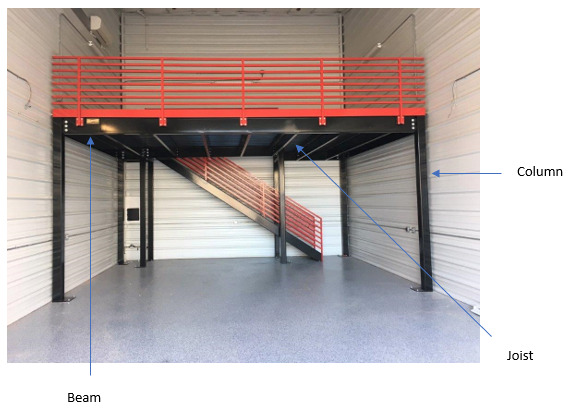
\includegraphics[width=\textwidth]{Images/General/mz.jpg}
\caption{Mezzanine parts. \vspace{0.5cm} Source: http://www.firststorage.co.za}
\label{mezzanine}
\end{figure}

\vspace{-0.7cm}

The resistance of a structural member rely on the material, geometry of the section and the length of the member. By default, the framework is programmed to work with steel ASTM A1011 SS Grade 36/2, which has the properties shown on Table \ref{properties}.

\begin{table}[h!]
\centering
\begin{adjustbox}{max width=\textwidth}
\begin{tabular}{c c}
\hline
\textbf{Parameter} & \textbf{Value} \\ \hline
Density $\left[kg/m^3\right]$ & 7850 \\ \hline
Young Modulus $[GPa]$ & 200 \\ \hline
Coefficient of Poisson & 0.3 \\ \hline
Yield strength $[MPa]$ & 248.25 \\ \hline
Ultimate strength $[Mpa]$ & 440 \\ \hline
\end{tabular}
\end{adjustbox}
\caption{Strength properties.}
\label{properties}
\end{table}

Other materials can be defined and selected by the user, even composite cross sections can be implemented.
 
 



%\section{Design methodology}

The established methodology proposed can be appreciated on Figure \ref{methodology}.

% Define block styles: decision, block, line, cloud, blockTwo
\tikzstyle{decision} = [diamond, draw, fill=blue!20, 
       text width=7em, text badly centered, node distance=3cm, inner sep=0pt]
\tikzstyle{block} = [rectangle, draw, fill=blue!20, 
       text width=7em, text centered, rounded corners, minimum height=4em]
\tikzstyle{blockConc} = [rectangle, draw, fill=orange!20, 
       text width=7em, text centered, rounded corners, minimum height=4em]
\tikzstyle{empty} = [rectangle, draw, white, fill=white, 
       text width=-4em, text centered, rounded corners, minimum height=-4em]
\tikzstyle{line} = [draw, -latex']
\tikzstyle{cloud} = [draw, ellipse,fill=red!20, node distance=3cm,
       minimum height=2em]
\tikzstyle{blockTwo} = [rectangle, draw, fill=blue!20, 
       text width=3em, text centered, rounded corners, minimum height=4em]

\begin{figure}[h!]
\centering
\begin{adjustbox}{max width=\textwidth}
\begin{tikzpicture}[scale=1, node distance = 1cm]
       % Place nodes
       \node [block] (init) {Material selection};
       \node [block, below of=init, node distance=3cm] (reco) {Cross section database definition};
       \node [block, below of=reco, node distance=3cm] (velsed) {Definition of the area of the structure and load conditions};
       \node [block, below of=velsed, node distance=3cm] (geo) {Structural design procedure};
	   \node [blockConc, below of=geo, node distance=4cm] (conc) {Engineering report, cost analysis and CAD drawings };     
       
       %\draw (-1.58,-16) -- (-2.5,-16) -- (-2.5, -3) -- (-1.58,-3);
       
       %\node [left of=decide, node distance = 2.5cm] (intermedio)
       % Draw edges
       \path [line] (init) -- (reco);
       \path [line] (reco) -- (velsed);
       \path [line] (velsed) -- (geo);
       \path [line] (geo) -- (conc);
       %\path [line] (res.west) -- (decide.west);
\end{tikzpicture}
\end{adjustbox}
\caption{Working methodology.}
\label{methodology}
\end{figure}
\section{Cross Sections}

To predict the cross section properties, iStructure implements the \textit{section properties} Open Source library \cite{secprop}. With the material of the structural members chosen, the next step should be to establish a database of structural profiles. By default, the software use square sections for columns, I section for beams and C section for joists. Other kinds of sections are also supported, including user custom sections. For example, for a joist, Cee section, you simply specify the dimensions, as shown on Listing 1.

\begin{lstlisting}[language=Python, caption=Cee section definition]
from sectionproperties.pre.sections import CeeSection
cee = CeeSection(d=120, b=60, l=15, t=4, r_out=5.4, n_r=8)
cee.plot_geometry()
\end{lstlisting}

Cee cross section scheme can be appreciated on figure \ref{cScheme}.

\begin{figure}[h!]
\centering
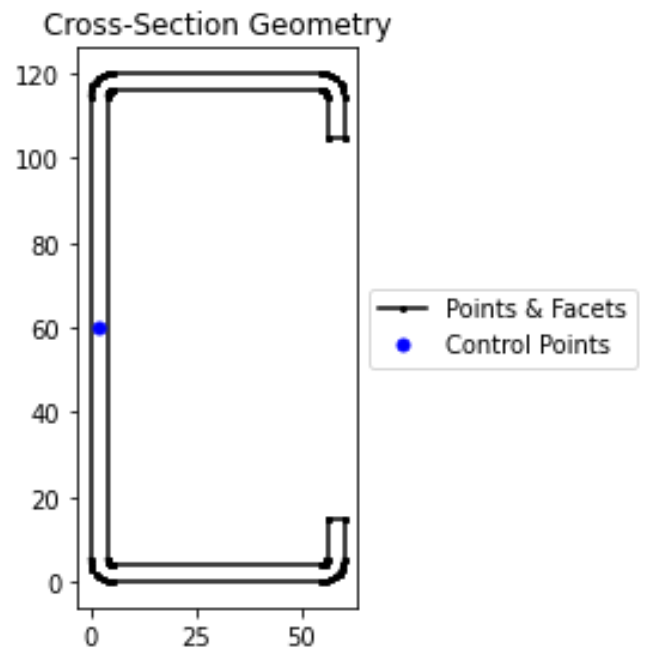
\includegraphics[width=0.8\textwidth]{Images/sections/cee.PNG}
\caption{Cee section.}
\label{cScheme}
\end{figure}

Geometric, plastic and warping analysis is developed by a Finite Element Method simulation of the cross section. We start by applying the discretization of the domain.

\begin{lstlisting}[language=Python, caption=Cee section definition]
from iStructure.CrossSection.MechProp import CrossSection
from iStructure.CrossSection.GenericMaterials import steel
mesh = cee.create_mesh(mesh_sizes=[3.0])
ceeSection = CrossSection(cee, mesh, [steel])
ceeSection.display_mesh_info()
\end{lstlisting}

With this configuration, a regular tetrahedral mesh, with elements of $3[mm]$ has been developed and can be appreciated next.

\begin{figure}[h!]
\centering
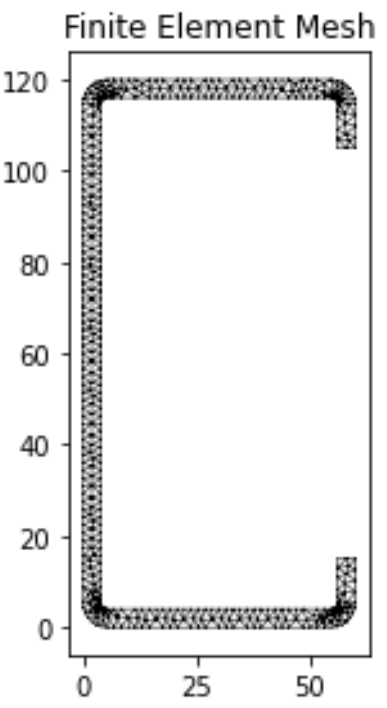
\includegraphics[width=0.45\textwidth]{Images/sections/ceeMesh.PNG}
\caption{Cee section mesh.}
\label{cMesh}
\end{figure}

\subsection{Cross section properties and FEM formulation}

\vspace{0.5cm}

\subsubsection{Problem statement}

The geometrical and wrap properties are calculated by the Finite Element Method. For the 2D linear elasticity problem, the unknown displacement field $u$, taking values in $\Omega \subset \mathbb{R} ^2$, is the solution of the boundary value problem, given by:

\begin{equation}
- \nabla \cdot \sigma (u) = b \quad \quad \quad \quad  \text{in } \Omega
\end{equation}

\begin{equation}
\sigma (u) \cdot n = t \quad \quad \quad \quad \quad  \text{on } \Gamma _N
\end{equation}

\begin{equation}
u = 0 \quad \quad \quad \quad \quad \quad \quad \text{on } \Gamma _D
\end{equation}

Where $\Gamma _N$ and $\Gamma _D$ denote the Neumann and Dirichlet boundaries with $\partial \Omega = \Gamma _N \cup \Gamma _D$  and $\Gamma _N \cap \Gamma _D = \emptyset$. The Dirichlet boundary condition in (3) is assumed to be homogeneous. The weak form of the problem reads: Find $u \in V$ sucha that

\begin{equation}
\forall v \in V \quad \quad \quad a (u,v) = l(v)
\end{equation}

where V is the standard test space for the elasticity problem such that $V = {v | v }$, and 

\begin{equation}
	a (u,v) = \int _\Omega \epsilon (u ) ^T D \epsilon (v) d \Omega = \int _\Omega \sigma (u)^T D ^{-1} \sigma (v) d\Omega
\end{equation}

\begin{equation}
l (v) := \int _\Omega b^T v d\Omega + \int _{\Gamma _N} t^T v d \Gamma
\end{equation}

where $D$ is the elasticity matrix of the constitutive relation $\sigma = D \epsilon$, $\sigma$ and $\epsilon$ denote the stress and strain operators.

\subsubsection{Finite element formulation}

Let $u ^h$ be a finite element approximation to $u$. The solution lies in a functional space $V ^h \subset V$ associated with a mesh of isoparametric finite elements of characteristic size h, which is defined by equation (3). 

Using a variational formulation of the problem (1-3) and a finite element approximation $u^h = N u^{e}$, where $N$ denotes the shape functions of order $p$, we obtain a system of linear equations to solve the displacements at nodes $u^e$:

\begin{equation}
K U = f
\end{equation}

where $K$ is the stiffness matrix, $U$ is the vector of nodal displacements and $f$ is the load vector.


\subsection{NN mesh validation}

For mesh validation error, an internal neural network algorithm has been implemented.
\section{Area distribution}

The modular distribution of the structure is automated by an algorithm from which the user can interact directly by telling the software the general dimensions (width, height and length), separation between joists, modular subdivisions and load distribution. Moreover, it was designed to be flexible enough to adapt for complex geometries. For example, lets suppose that a client has a warehouse of six by six meters of area and wants a structure with three meters of height which has to support $700 \left[kg/ m^2 \right]$, but the building has a column in the middle of it with square dimensions of $0.5 [m]$. A possible solution for this problem can be appreciated on Figure \ref{area}.

\vspace{-0.7cm}

\begin{figure}[h!]
\centering
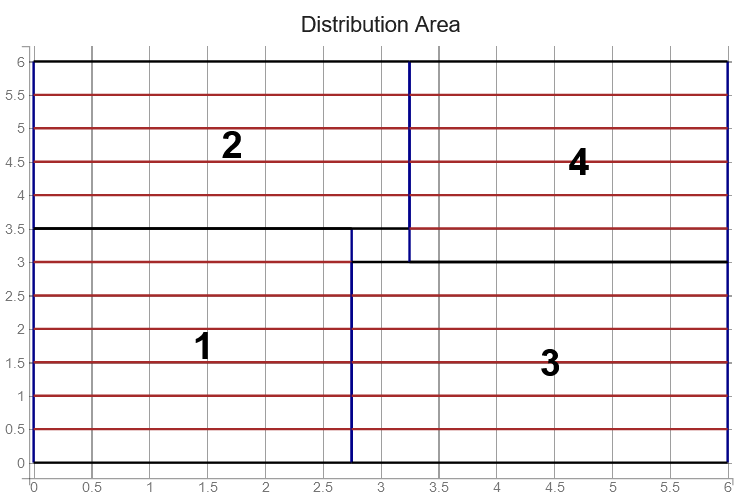
\includegraphics[width=0.9\textwidth]{Images/General/area2.PNG}
\caption{Area distribution of study.}
\label{area}
\end{figure}

\vspace{-0.7cm}

As seen on Figure \ref{area2}, an algorithm of \textit{Object Oriented Programming} (OOP) has been implemented to the automatic distribution of the area, using RAM memory\footnote{Off course, this can be changed to be stored on the HDD memory rather than RAM memory, if needed.} to store the dimensions of each module, in this case: 1, 2, 3 and 4. An object of the module was created which uses $x$ and $y$ position to know its position in the space, $L$ and $W$ parameters referring to \textit{length} and \textit{width}, respectively, and a `Delete' checkbox to erase the module (not used in this example).

\begin{figure}[h!]
\centering
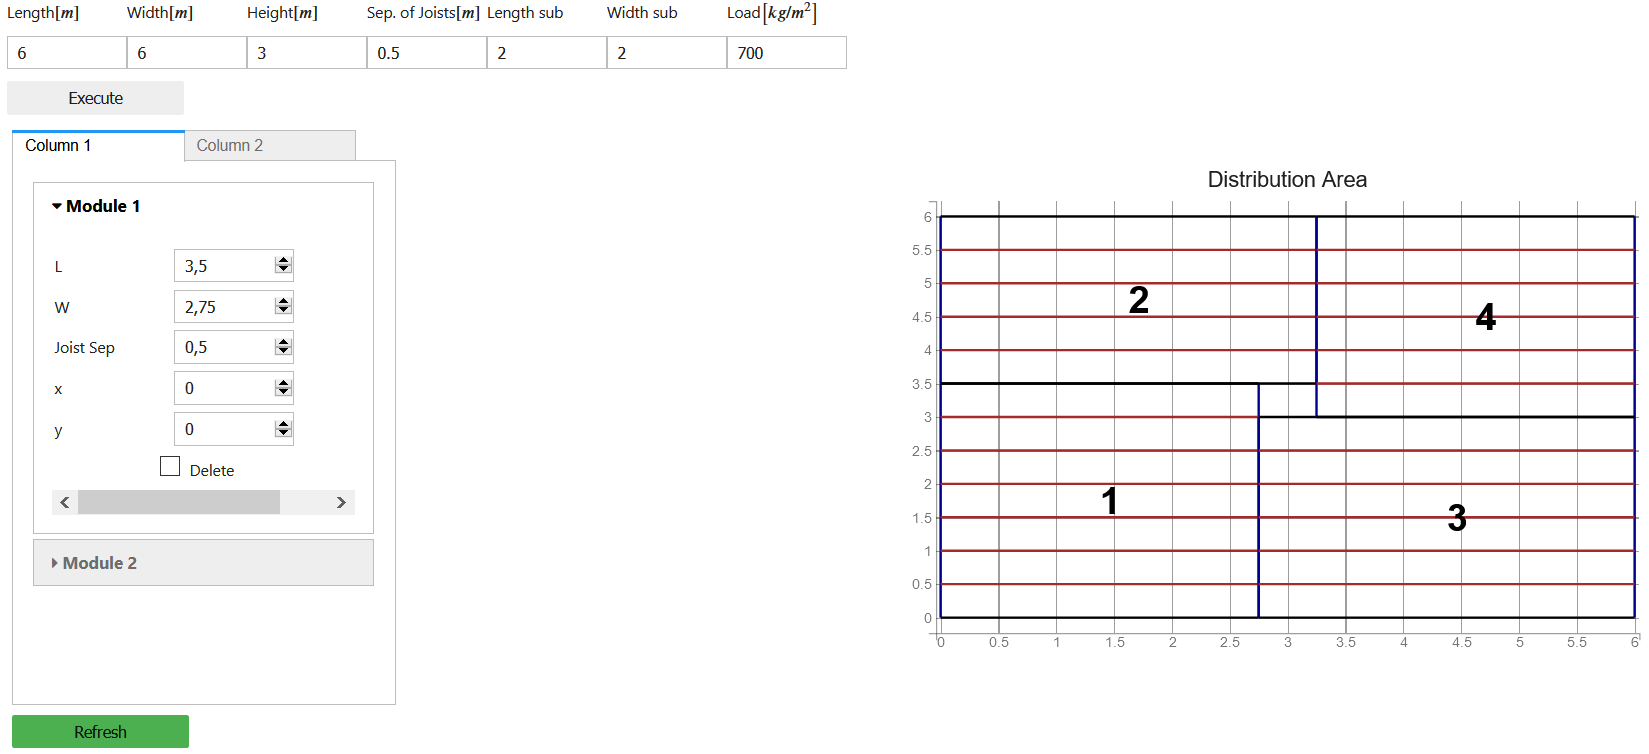
\includegraphics[width=0.88\textwidth]{Images/General/area.PNG}
\caption{User interface of the area distribution.}
\label{area2}
\end{figure}
\section{Structural members selection procedure}

To start the structural members selection, it is needed to be known the longest dimensions of each member. It can be achieved by implementing an algorithm which compares all the dimensions of each module. All of this information has been stored in a Python dictionary.

\subsection{Load study}

As defined on AISI S100-16 standard, load distribution can be segmented in \textit{dead}, \textit{live}, \textit{product} and \textit{combined} loads. 

\subsubsection{Dead load}

It consists of the weight of the structural members. It depends on the densisty of the material, the cross sectional area and the length of the member.

\begin{equation}
    D = A \rho L g
    \label{eq:dead}
\end{equation}

From Equation $\eqref{eq:dead}$, $D$ correspond to the value of the dead load, $A$ to the cross sectional area, $L$ to the length of the member and $g$ to gravity's acceleration.

\subsubsection{Live load}

The distirbuted live load for the food traffic on pick module walkways should be, at least, of $293 \left[kg / m^2 \right]$, according to the standard ANSI MH16, section 8.4.2. The live load can be calculated using Equation. $\eqref{eq:live}$.

\begin{equation}
    L = L_{dist} A g
    \label{eq:live}
\end{equation}

 Where: $L$ is the live load, $L_{dist}$ is the distributed load, $A$ correspond to the area of the biggest module and $g$ to the gravity.

\subsubsection{Product load}

The product load correspond to the difference between the design distributed load, the live load and the dead load.

\subsubsection{Combined load}

The combined load is used to determine the stresses of the structural members. There was used a Load and Resistance Factor Design (LRFD, ANSI MH16.1 section 2.1) as seen on Equation $\eqref{eq:combinedload}$.

\begin{equation}
    CL = 1.2 D + 1.4 P +1.6 L
    \label{eq:combinedload}
\end{equation}

Where: $CL$ is the combined load, $D$ is the dead load (Eq. $\eqref{eq:dead}$), $P$ is the product load and $L$ is the live load (Equation $\eqref{eq:live}$).

\subsection{Joists}

Structural design of joists is evaluated based on the maximum momentum compared \textit{nominal resistance momentum} (section 3.3.2.2.2 of AISI S100-16 standard).

\begin{figure}[h!]
\centering
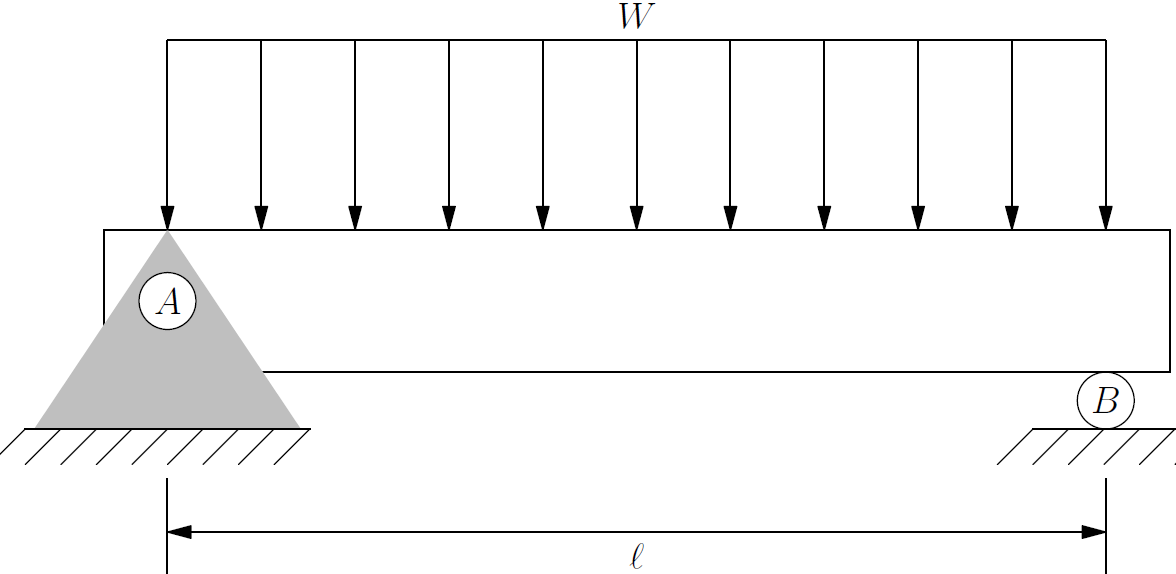
\includegraphics[width=\textwidth]{Images/Calculus/Vigueta/Vigueta.PNG}
\caption{Load distribution over a joist.}
\label{distjoist}
\end{figure}

As it can be appreciated on Figure \ref{distjoist}, the calculation proccess starts by the supposition of a simply supported beam. The distributed load $W$ correspond to the combined load, from Equation $\eqref{eq:combinedload}$. The momentum behaviour over the joist is defined by Equation $\eqref{eq:joistmoment}$.

\begin{equation}
M(x) = \frac{W x (L-x)}{2}
\label{eq:joistmoment}
\end{equation}

According to the Equation $\eqref{eq:joistmoment}$, the maximum momentum is:

\begin{equation}
M = \frac{W L^2}{8}
\end{equation}

\subsubsection{Selection}

Joist selection is developed by each of the structural profile in the database. For each of them is evaluated and compared both maximum momentum and nominal resistance momentum. The final selection is to the member with the lowest cross sectional area, for this example the summary table is shown on Figure \ref{joistselec}.

\begin{figure}[h!]
\centering
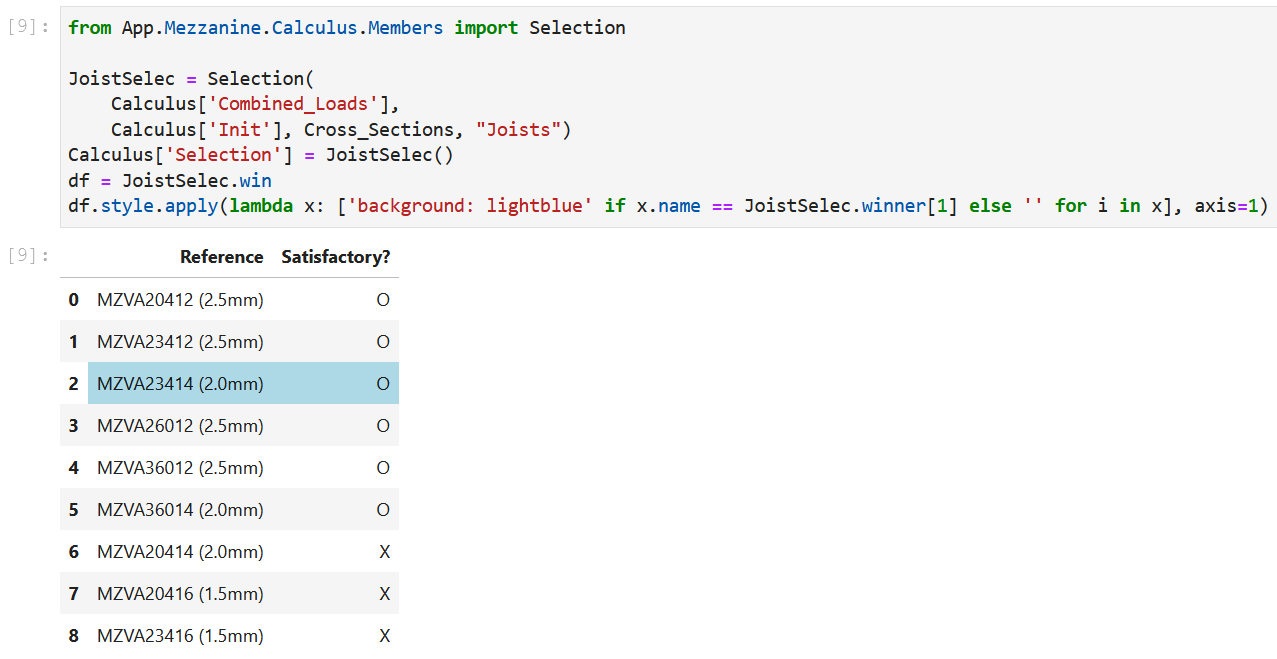
\includegraphics[width=\textwidth]{Images/Calculus/viguetaselec.PNG}
\caption{Selection table.}
\label{joistselec}
\end{figure} 

From Table \ref{joistselec}, the selected member is `MZVA23414 (2.0 mm)'.

\subsection{Beams}

The structural evaluation procedure is the same as joists (section 3.2).

\begin{figure}[h!]
\centering
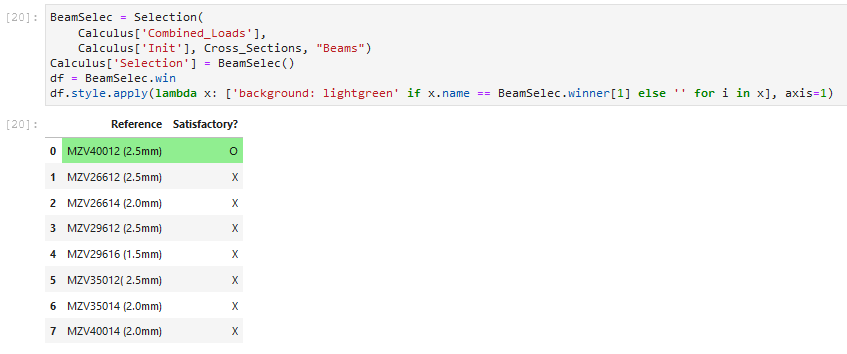
\includegraphics[width=\textwidth]{Images/Calculus/vigaselec.PNG}
\caption{Selection table for beams.}
\label{beamselec}
\end{figure} 

\subsection{Columns}

Unlike beams and joists, columns are multiaxial load members. When the column of a structure fails it is mainly because of flexural-torsional buckling stresses (`large' columns) or axial stresses (`short' columns). The procedure starts by evaluating compression load (axial stress) and compare it with the nominal load (result of the defined procedure given by the AISI S100-16 standard)  for each option of the database. If the nominal load has a bigger value than the calculated compression load, then it can be concluded that axial stress is not critical so the momentum due to flexural-torsional buckling should be compared with nominal momentum (defined by AISI S100-16 standard) to discard failure by buckling stresses. The results for the given example is shown on Figure \ref{column}.

\begin{figure}[h!]
\centering
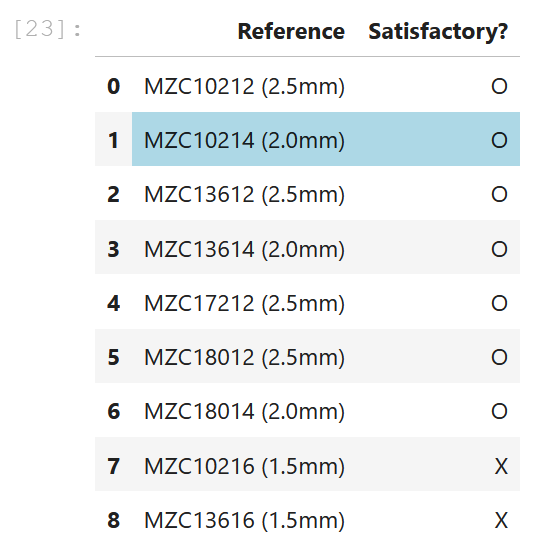
\includegraphics[width=\textwidth]{Images/Calculus/columnselec.PNG}
\caption{Column selection table.}
\label{columnselec}
\end{figure}

From Figure \ref{columnselec}, the column of reference `MZC10214' has been selected.
\begin{acknowledgment}
This creation was supported by Universidad Industrial de Santander (UIS). We thank our collegues from UIS who provided insight and expertise that greatly assisted this work. 
\end{acknowledgment}

\end{document}
